
\cleardoublepage


\chapter{Experimental Validation}




\section{Spectral Unfolding}

\subsection{Methods and Parameters}

% the responses and response functions were used with the unfolding methods described in ch2 to obtain solution spectra
The detector responses and response functions were unfolded with the methods described in chapter two to obtain a set of solution spectra.
% the bss and ft_au results were first considered separately, then combined
The responses from the foil tube and the BSS were first considered separetely, then combined into a single vector to produce a third spectrum for each unfolding method.
% both the gravel and maxed unfolding algorithms were used with these data
The Gravel, Doroshenko, and MAXED unfolding algorithms were used.
% for gravel, 50 iterations were used
For both Gravel and Doroshenko, the termination criteria was set at 50 iterations.
% for maxed, the parameter omega was set using the number of detectors for each dataset, 9 for the foil tube, 7 for the bss, and 16 for the combined set
For MAXED, the parameter Omega was set using the number of detectors for each dataset, 9 for the foil tube, 7 for the BSS, and 16 for the combined case.
% then, the maxed portion was repeated, while first scaling the default spectrum
Then, the MAXED unfolding was repeated, but with a scaled default spectrum.
In this case, scaled means that the default spectrum was normalized so the average of the computed responses was equal to the average of the experimentally obtained responses before unfolding.

\subsection{Results and Discussion}


\begin{figure}[htb]
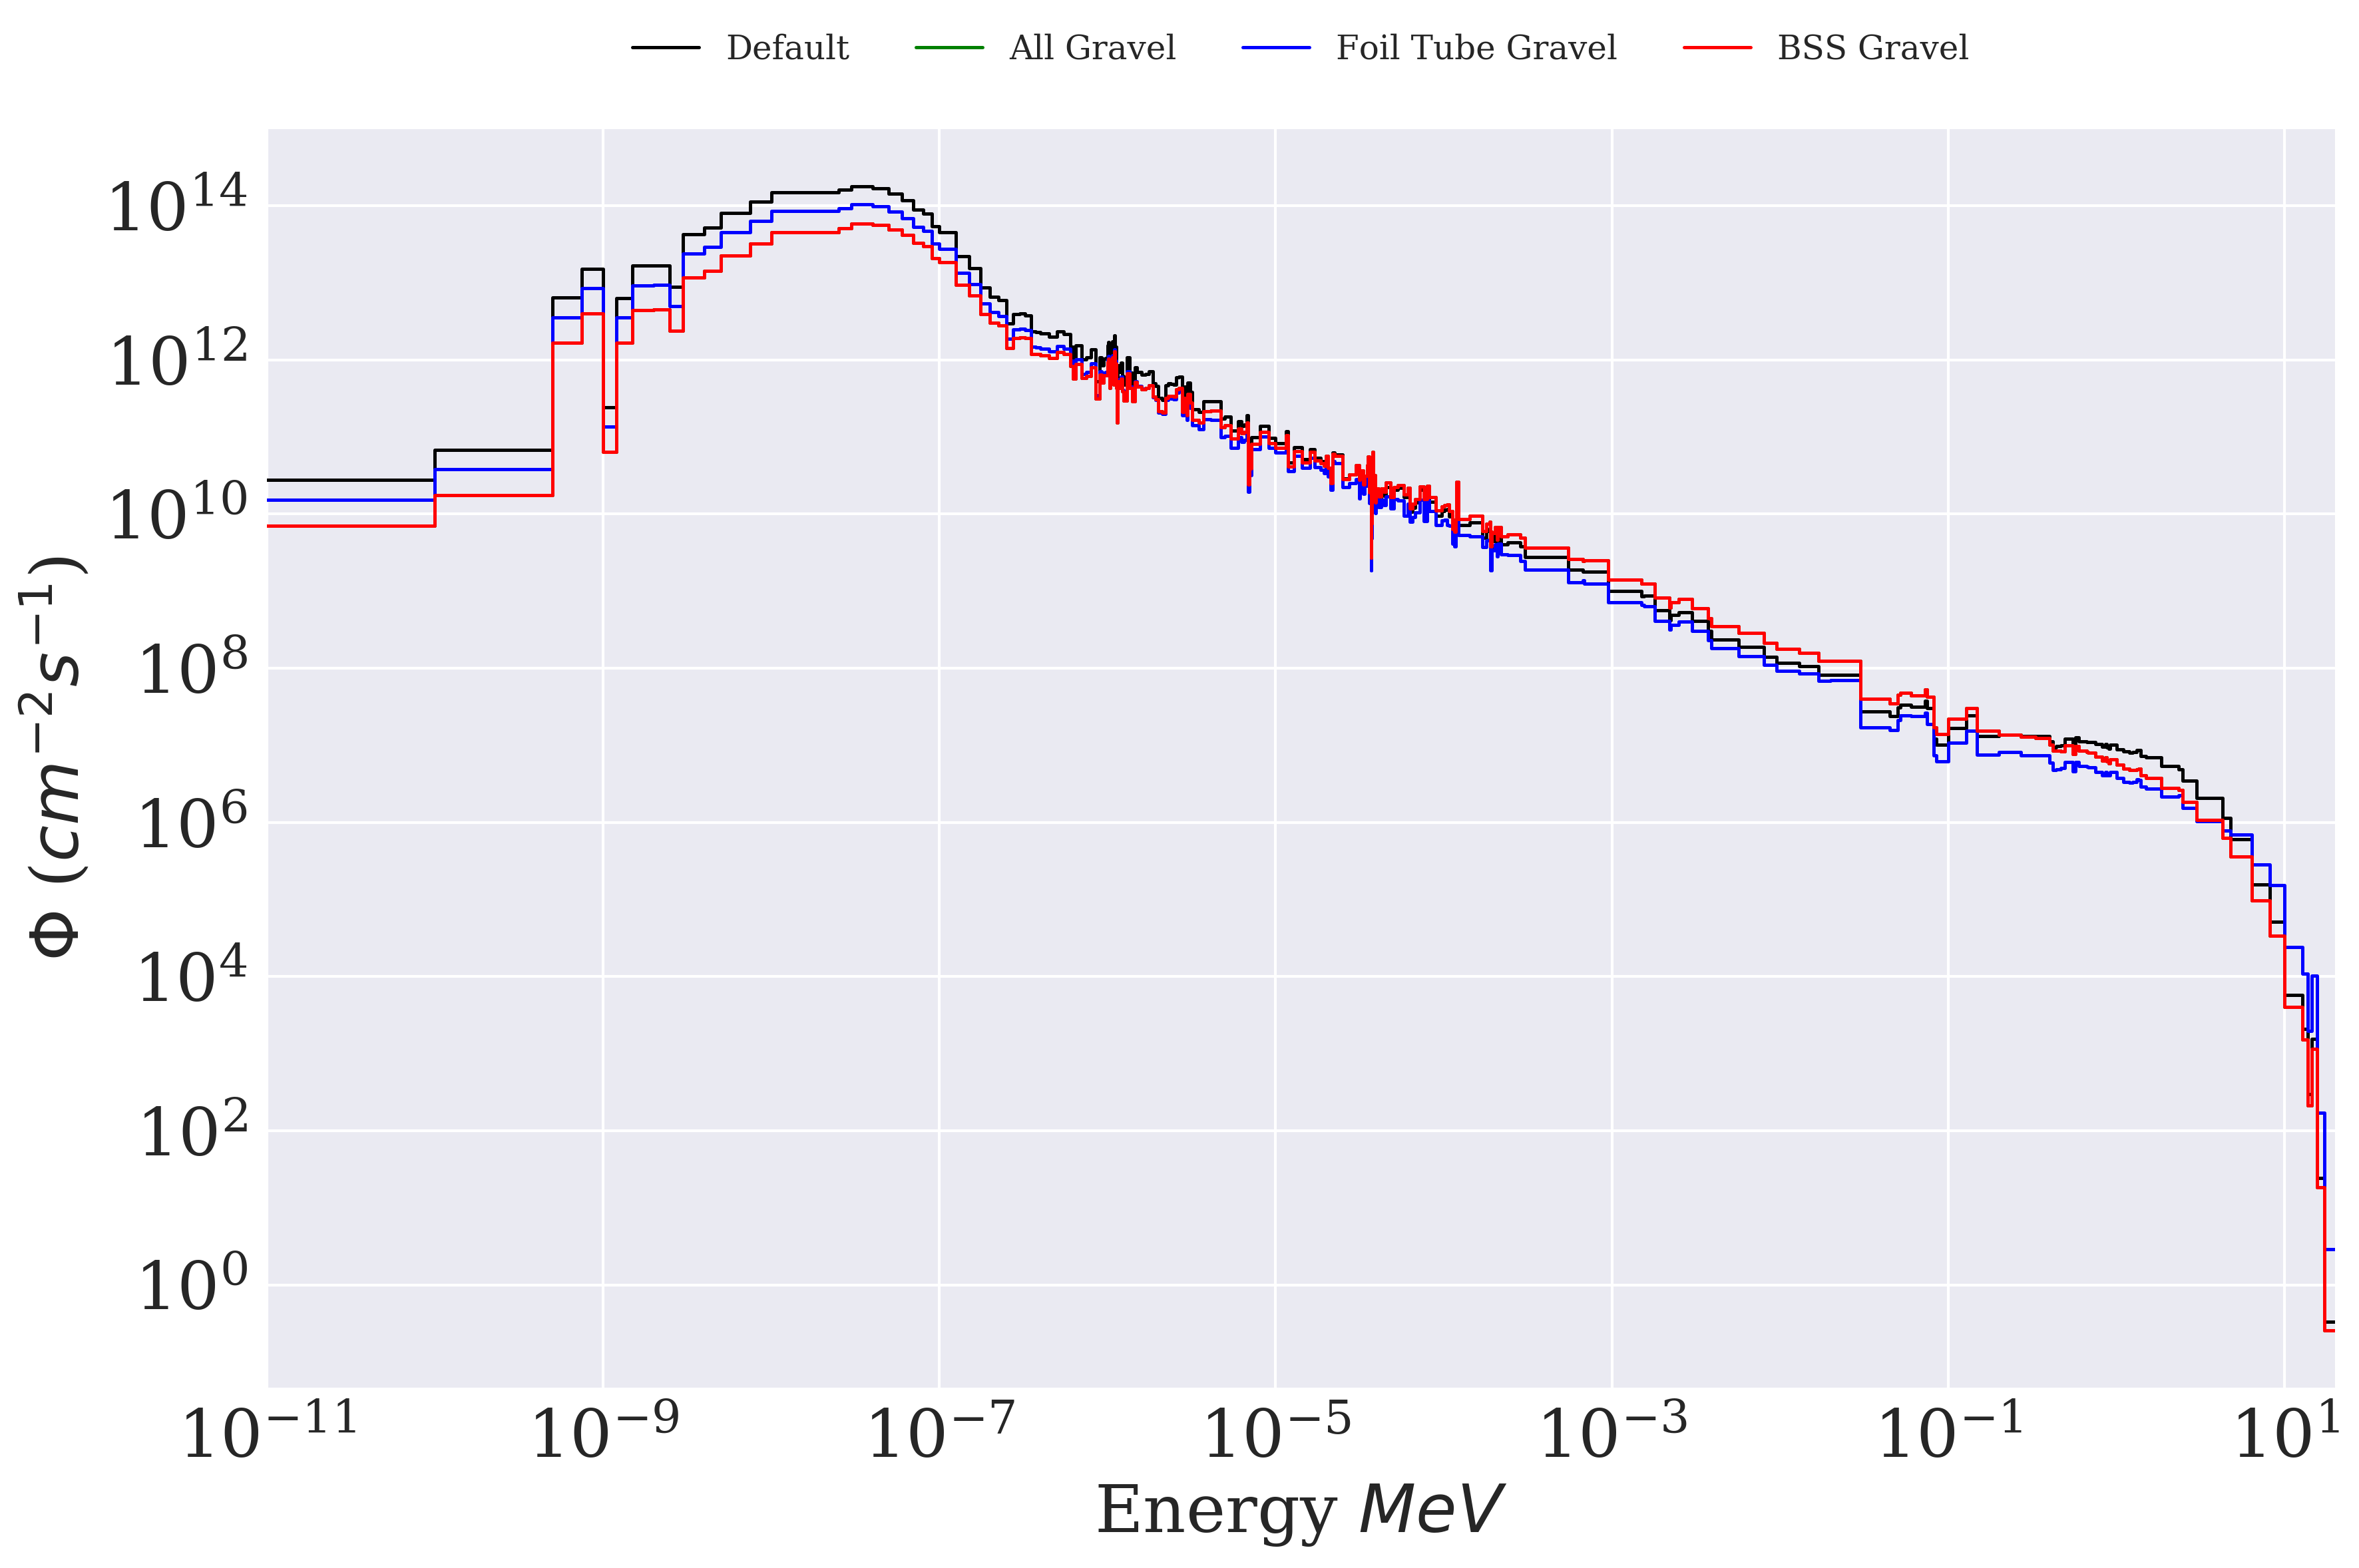
\includegraphics[height=3.8in]{tex/figures/unfolded_gr.png}
\caption[Gravel Unfolded Spectra]{The unfolded NEBP spectra obtained from using the Gravel method.}
\label{fig:unfolded_gr}
\end{figure}

% here gravel results are presented first
Here, the Gravel results are presented in \FIG{fig:unfolded_gr}
% as seen in the figure, the bss and ft_au results show good agreeance with one another
As seen in the figure, the foil tube and BSS results show good agreeace with one another.
% all of the major features from the default spectrum are preserved
All of the major features from the default spectrum are preserved.
% the ft_au results unfold to a slightly higher thermal flux than the bss where as the bss show slightly higher fast region
Some differences appear between the two datasets, where the foil tube shows a slightly higher thermal flux and the BSS is larger through a portion of the fast region.
% the combined results cannot be seen as they are covered by the ft_au
The combined results cannot be seen as they are covered by the foil tube data.
% this is because with gravel, smaller error responses are weighted heavier and the errors are much smaller for the gold foils than for the bss
This is due to the fact that the gravel algorithm will base its manipulation on relative error, meaning that smaller error (more well-known) responses will affect the final results more, and the errors from the foil tube are much smaller than the BSS results.

\begin{figure}[htb]
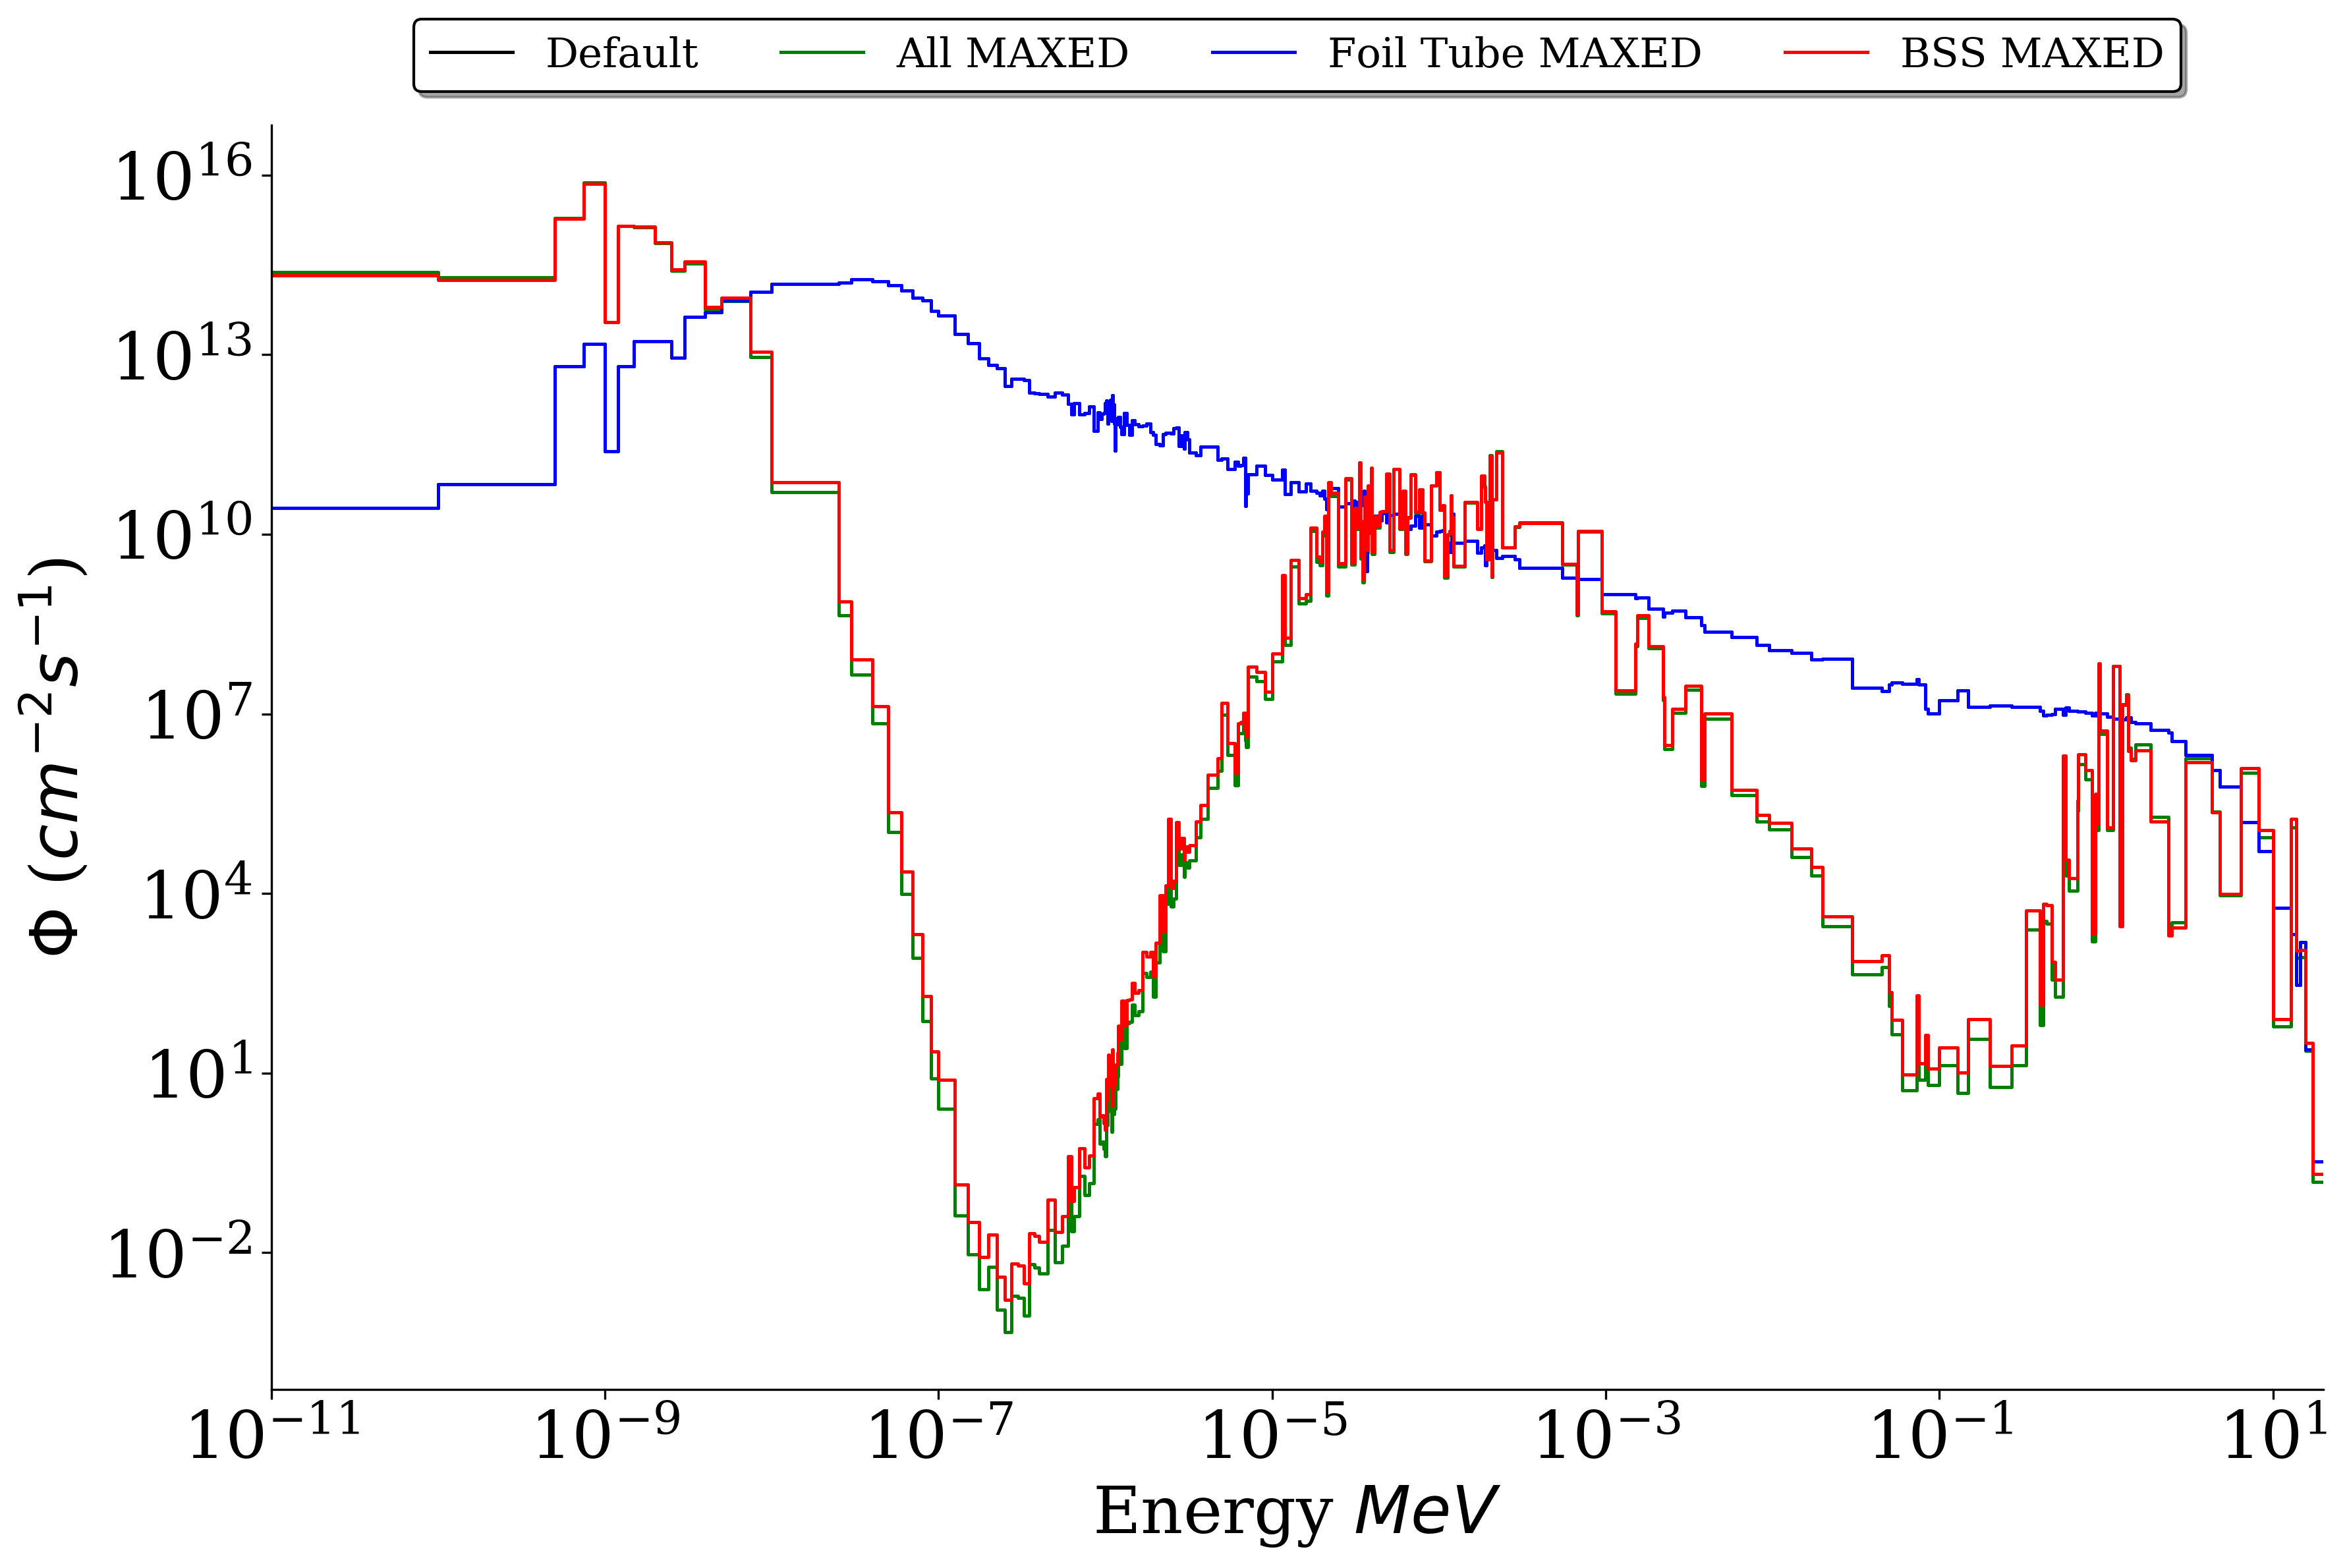
\includegraphics[height=3.8in]{tex/figures/unfolded_mx.png}
\caption[MAXED Unfolded Spectra]{The unfolded NEBP spectra obtained using the MAXED method.}
\label{fig:unfolded_mx}
\end{figure}

% these results shown in FIG are from the maxed unfolding.
Seen in \FIG{fig:unfolded_mx} are the results from the MAXED unfolding.
% in the case of the bss and combined case, the results produced are very unphysical
In the BSS and combined cases, the results produced appear very unphysical.
% this is likely due to the fact that the spectrum is trying to fit the data while staying close to the default spectrum
This is likely due to the fact that the algorithm is trying to fit the data while retaining some values close to the defaults spectrum to maximize the cross entropy between the two spectra.
% in the ft_au case, the default spectrum remains unchanged, indicating that the default spectrum actually represents a decent fit of the data
The default spectrum remains unchanged for the foil tube case, which indicates that the default spectrum actually represents a decent fit of the data, although it's still not as close as in the Gravel case.

\begin{figure}[htb]
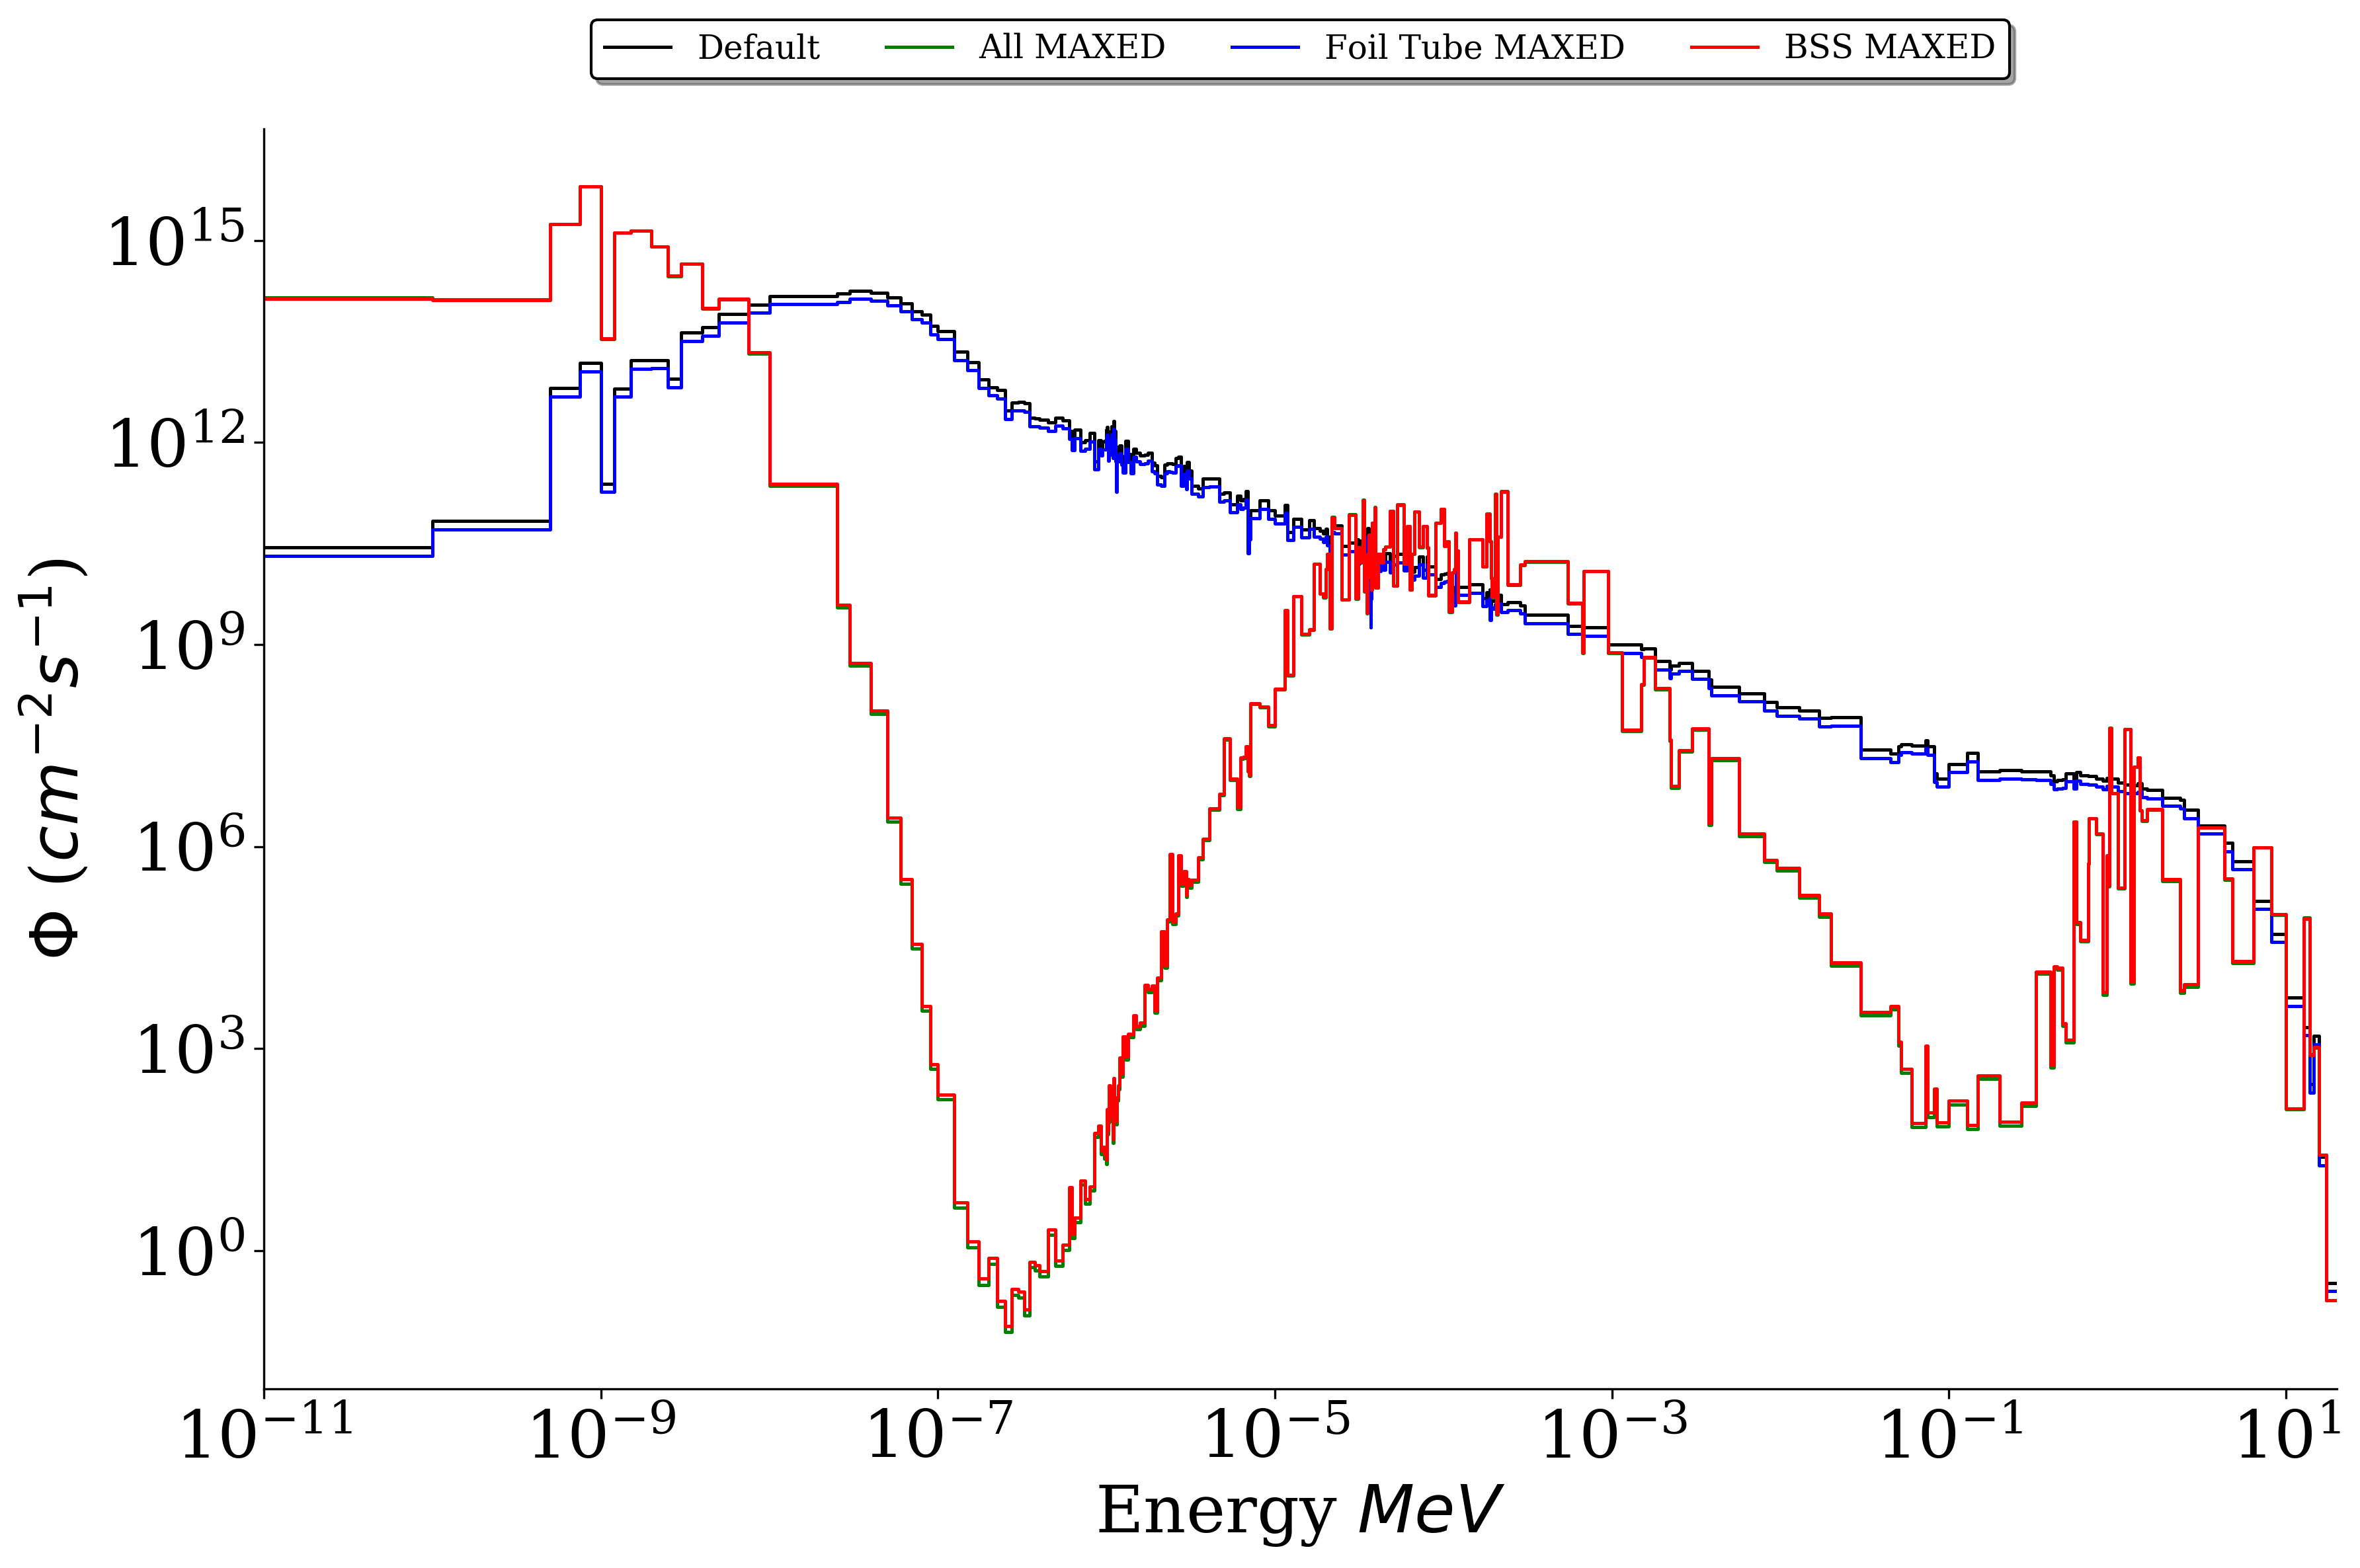
\includegraphics[height=3.8in]{tex/figures/unfolded_mx_sc.png}
\caption[MAXED Unfolded Spectra (Scaled)]{The unfolded NEBP spectra obtained from scaling the default spectrum then unfolding with the MAXED method.}
\label{fig:unfolded_mx_sc}
\end{figure}

% although it was hypothesized that scaling the spectrum would results in a less erratic answer, the results here are very similar in characteristics to the unscaled maxed results
It was hypothesized that scaling the defaults spectrum would remove some of the unphysicalities of the solution spectra; however, the results in \FIG{fig:unfolded_mx_sc} still appear erratic and are very similar in characteristics to the unscaled versions.
% the bss and combined cases are still unphysical, and the ft_au remaines unperturbed
The BSS and combined cases are still rather unphysical, and the foil tube solution remains unperturbed.

\begin{figure}[htb]
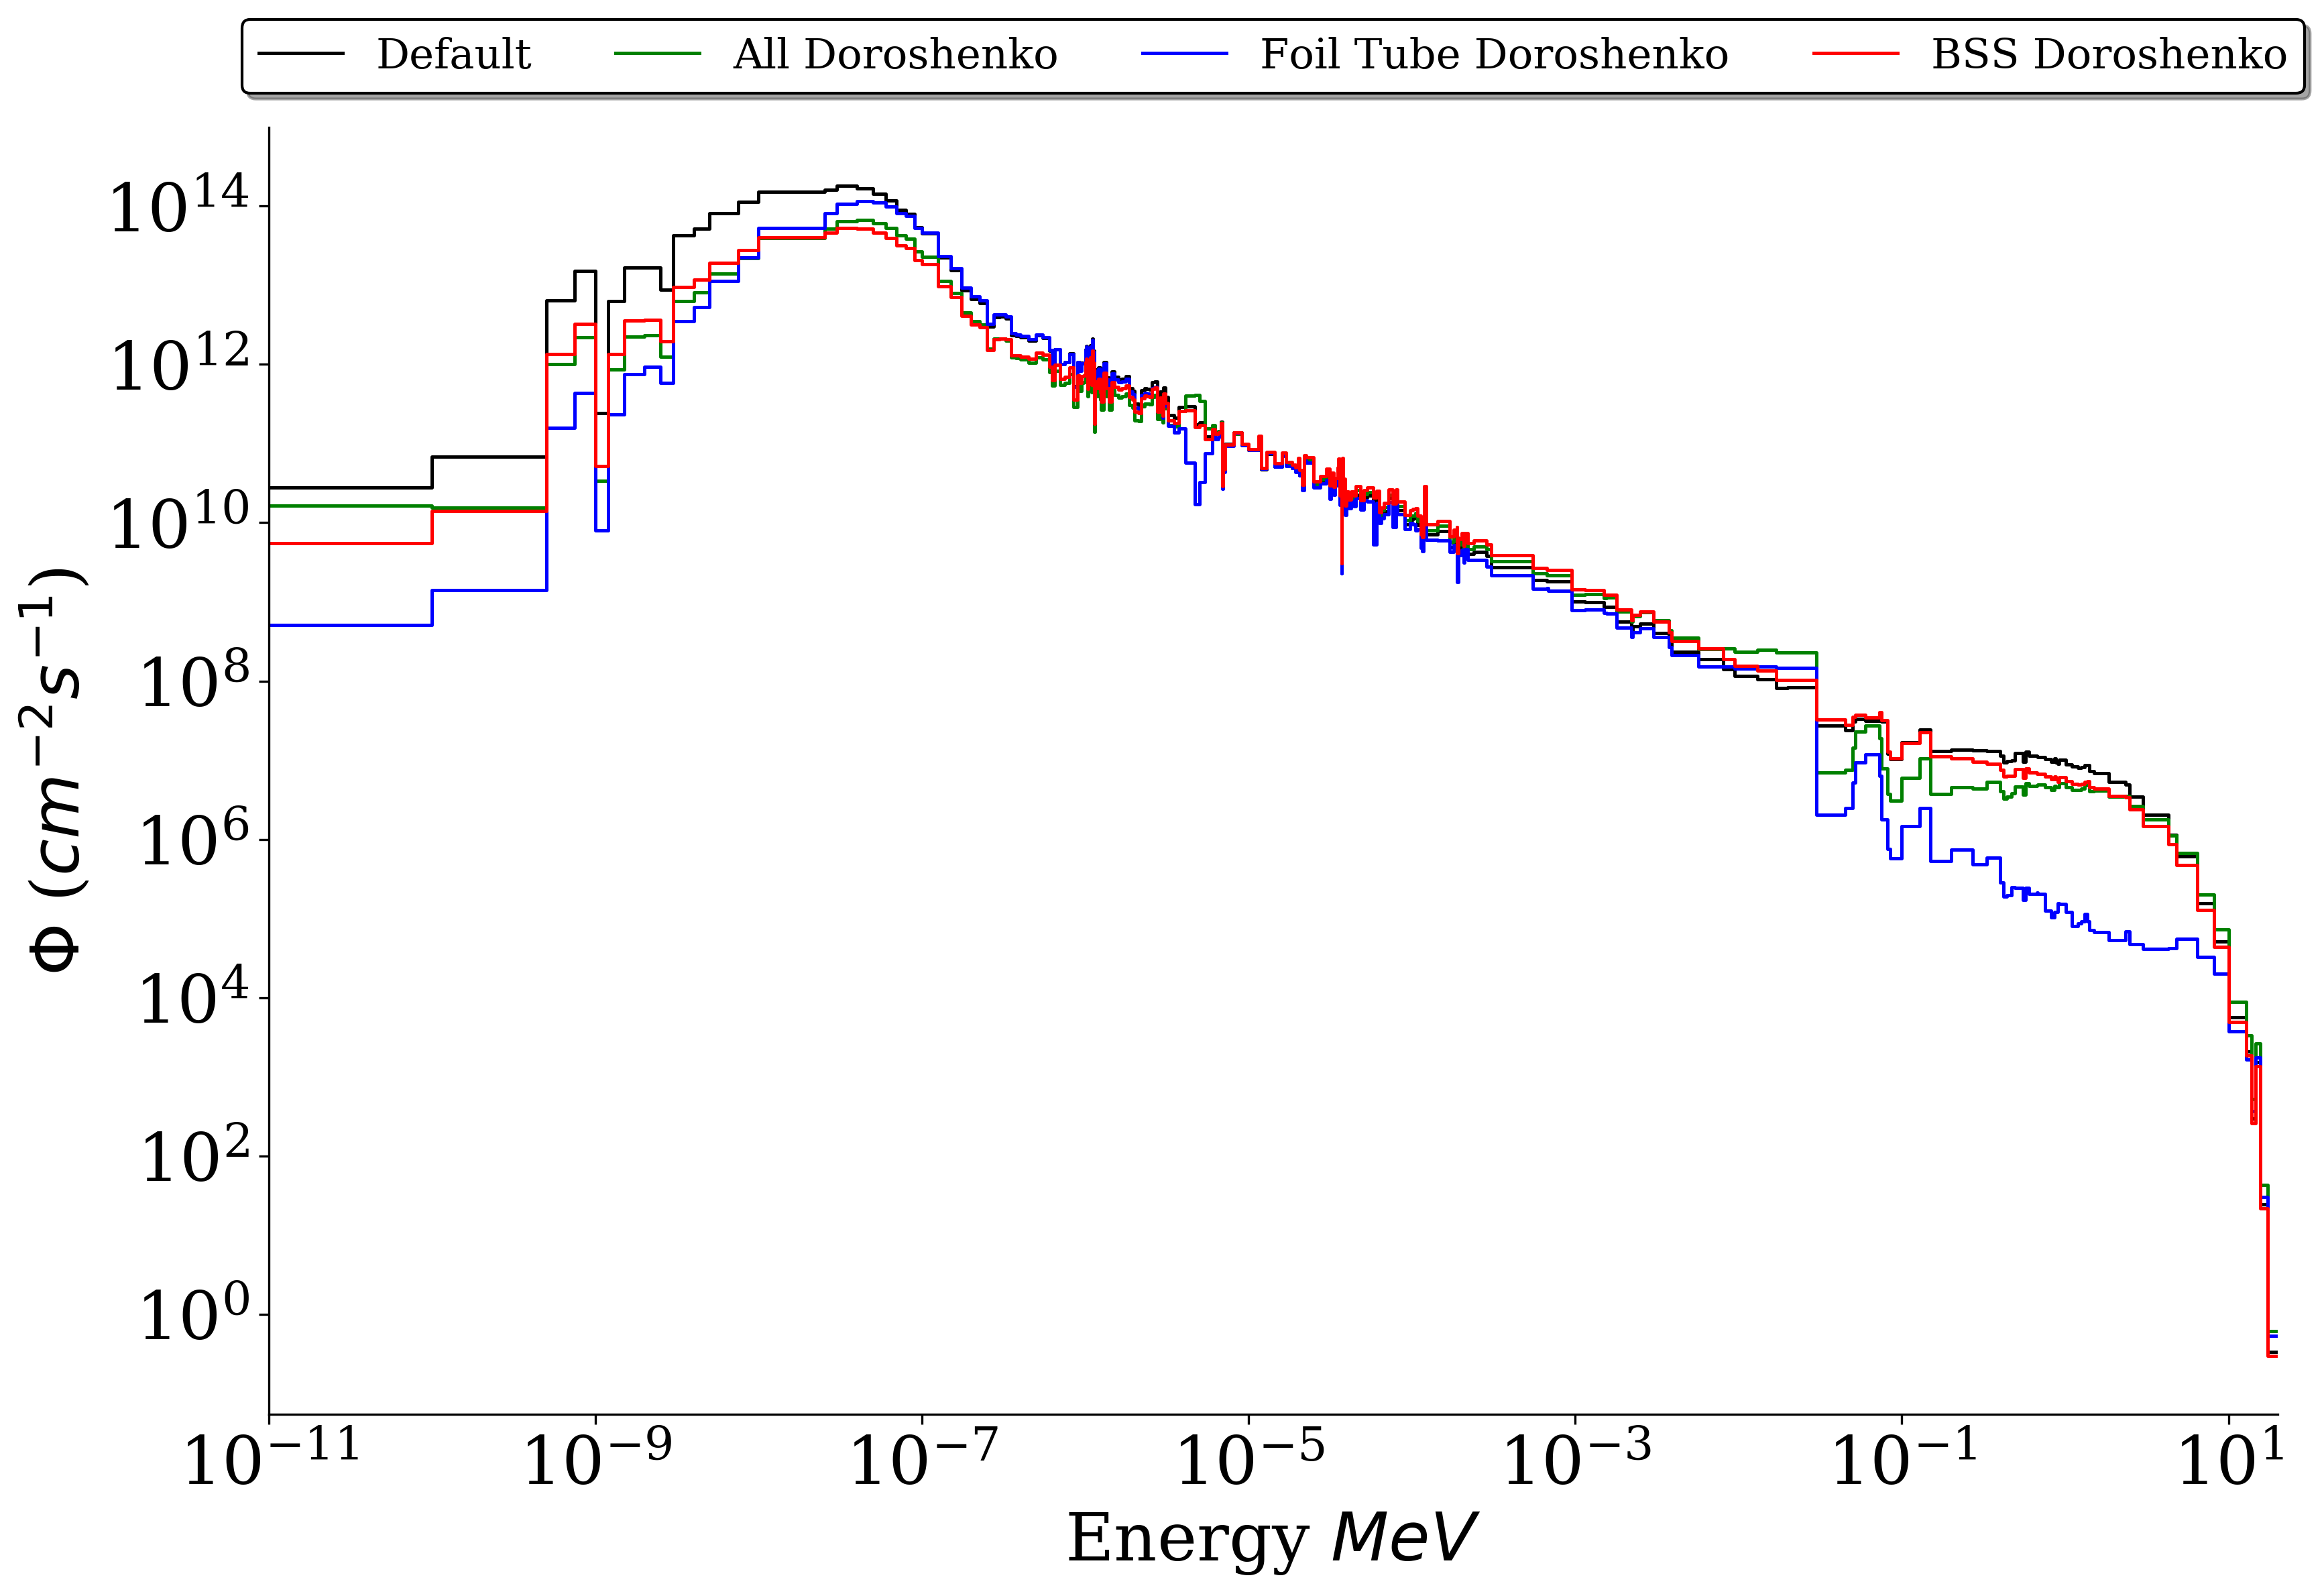
\includegraphics[height=3.8in]{tex/figures/unfolded_do.png}
\caption[Doroshenko Unfolded Spectra]{The unfolded NEBP spectra obtained from unfolding with the Doroshenko method.}
\label{fig:unfolded_do}
\end{figure}

% results in figure are from doroshenko
The results in \FIG{fig:unfolded_do} are from the Doroshenko unfolding.
% unlike maxed, they appear similar to the unfolding with gravel
Unlike MAXED, these results appear stable, like the Gravel data.
% here, though, the differences in the datasets are exemplified
Here, though, the differences between the datasets are more exemplefied.
This is most obvious in the foil tube dataset.
The fast end of the spectrum appears flattened as it tries to fit some of the foil data whose responses lie in that end.
Those responses have high error and likely this feature is due to a bias in the measurement, and not an actual spectral feature.
The other two datasets unfolded into reasonable-appearing spectra, with some slight variation in both the center of the maxwellian distribution, as well as in the flatness of the fast region.

